% Dyed-fabric atlas outputs (generated by toy_models/visualize_dyed_spacetime.py)
%
% Full multi-page PDF atlas (one galaxy per page):
%   toy_models/out_dyed_spacetime/dyed_spacetime_pages.pdf
%
% Contact sheet PDF (many galaxies per page):
%   toy_models/out_dyed_spacetime/dyed_spacetime_contact.pdf
%
% Individual PNGs:
%   toy_models/out_dyed_spacetime/png/<GALAXY>.png

% Example: include the contact sheet (fast overview)
\begin{figure}[t]
  \centering
  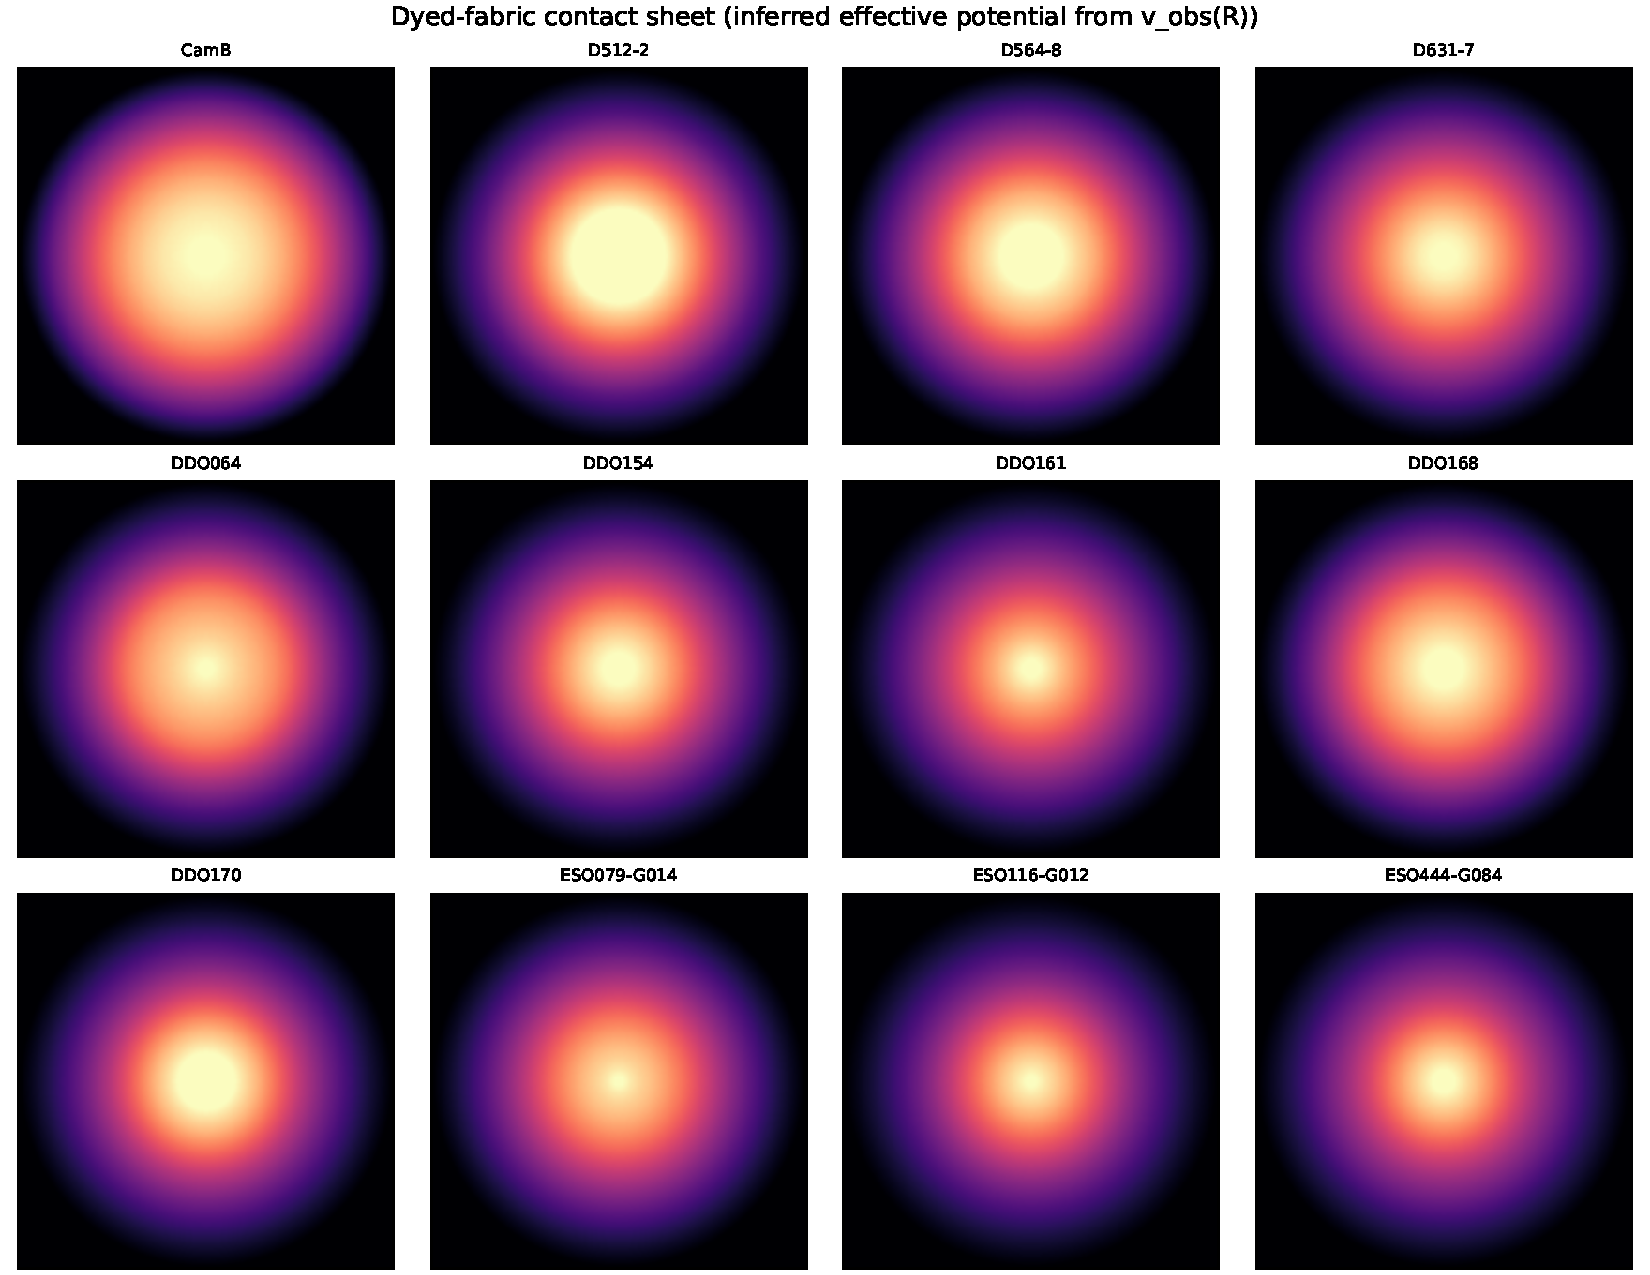
\includegraphics[width=\linewidth]{toy_models/out_dyed_spacetime/dyed_spacetime_contact.pdf}
  \caption{Dyed-fabric visualization inferred from observed rotation curves $v_{\mathrm{obs}}(R)$.
  The dyed panel encodes a normalized depth proportional to $-\int (v_{\mathrm{obs}}^2/R)\,dR$.
  This is a stylized effective-potential map for comparison across galaxies; it is not a GR embedding diagram and does not compute geodesics in a reconstructed metric.}
  \label{fig:dyed-fabric-contact}
\end{figure}

% Example: include a single galaxy PNG
% \begin{figure}[t]
%   \centering
%   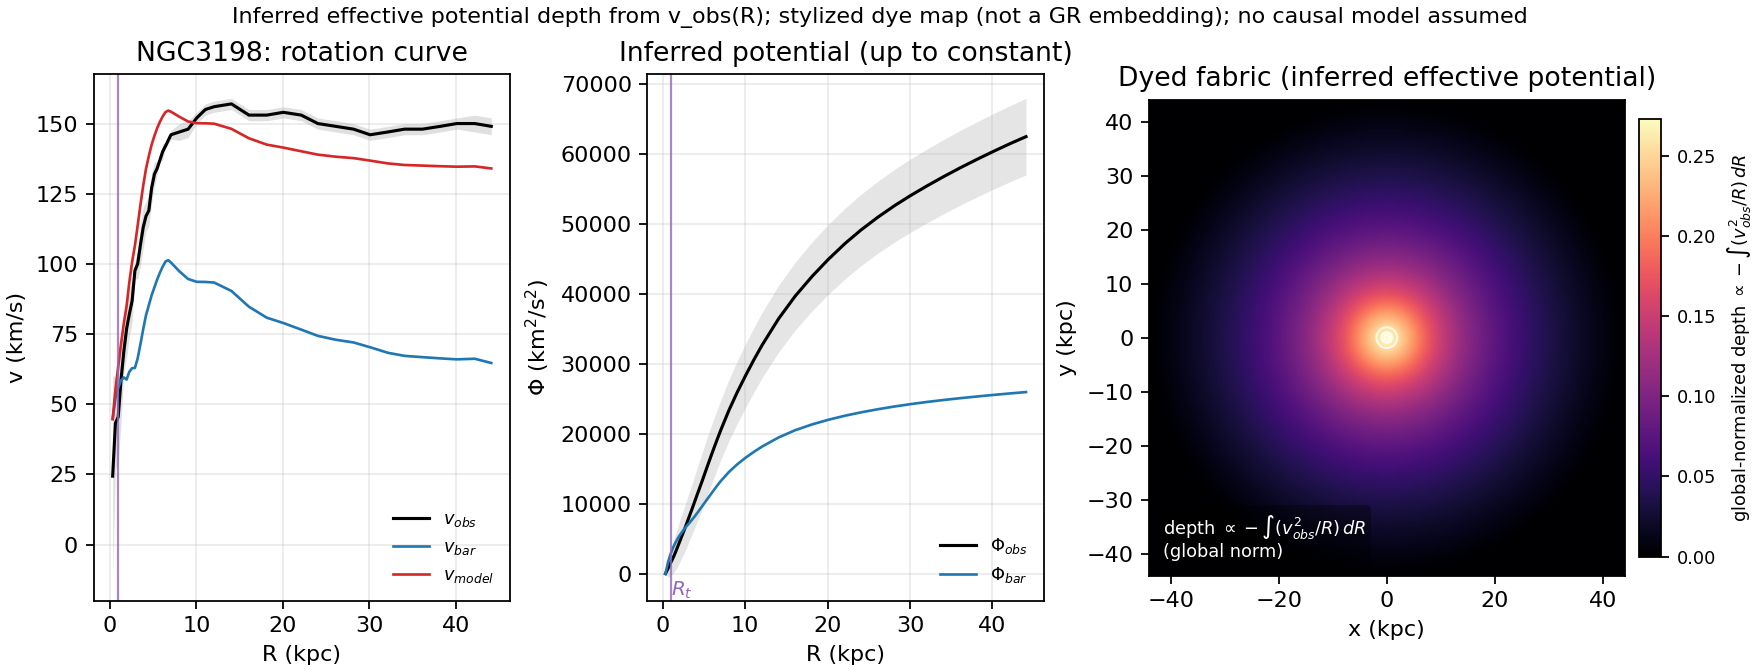
\includegraphics[width=0.95\linewidth]{toy_models/out_dyed_spacetime/png/NGC3198.png}
%   \caption{Example dyed-fabric figure for NGC3198.}
%   \label{fig:dyed-fabric-ngc3198}
% \end{figure}
